\documentclass[12pt]{article}

%% preamble: Keep it clean; only include those you need
\usepackage{amsmath}
\usepackage[margin = 1in]{geometry}
\usepackage{graphicx}
\usepackage{booktabs}
\usepackage{natbib}
\usepackage{float}

% for space filling
\usepackage{lipsum}
% highlighting hyper links
\usepackage[colorlinks=true, citecolor=blue]{hyperref}


%% meta data

\title{Statistical Properties of Loss Functions in Regression Model}
\author{Ge Li\\
  Department of Statistics\\
  University of Connecticut
}

\begin{document}
\maketitle


\paragraph{Introduction}
The advent of machine learning has profoundly impacted a wide array of disciplines, particularly emphasizing the pivotal role of loss functions in regression analysis. These functions not only quantify the discrepancy between predicted outputs and actual values but also fundamentally shape the learning process of algorithms. In the context of regression, loss functions such as Mean Squared Error (MSE) and Mean Absolute Error (MAE) are instrumental in the optimization of models, with their selection reflecting underlying assumptions about data distribution and noise characteristics \cite{hastie2009elements}. The selection of a loss function is a crucial decision that encapsulates the objectives and expectations of a model, particularly in terms of its robustness and generalization capabilities \cite{friedman2001elements}. The exploration of loss functions extends beyond traditional forms, with the Huber loss and other variants offering a middle ground between the sensitivity of MSE and the outlier robustness of MAE \cite{huber2011robust}. As machine learning applications become increasingly prevalent in high-stakes domains such as healthcare and finance, the implications of choosing an appropriate loss function cannot be understated, with the potential for significant consequences based on these decisions \cite{murphy2012machine}. This paper aims to conduct a thorough investigation into the statistical properties of loss functions utilized in regression tasks, dissecting the reasons behind their resilience or vulnerability to data anomalies. We seek to illuminate how these properties correspond with theoretical assumptions and practical performance, thereby equipping practitioners with the knowledge to tailor models that are both theoretically sound and empirically robust.


\paragraph{Data}
Our investigation leverages the esteemed Wine Quality Dataset, an invaluable resource in the realm of predictive modeling and sensory analysis. This dataset was meticulously curated by Paulo Cortez and his team at the University of Minho, Portugal, in collaboration with the Vinho Verde Commission of Viticulture (CVRVV)~\citep{wine_quality_source}. The database comprises two distinctive subsets: a collection of 1,599 red wine instances and a larger assemblage of 4,898 white wine instances. It effectively bridges the gap between objective tests, manifesting as physicochemical attributes, and subjective evaluations - the wine quality scores provided by seasoned wine experts.

To guarantee precision and address the multifaceted nature of wine evaluations, the wines in the dataset underwent rigorous physicochemical testing, resulting in a detailed profile of 11 key attributes. These attributes, ranging from fixed acidity and pH values to alcohol content, serve as the input variables. Complementing these, the output variable manifests as the quality score, a median rating obtained from at least three expert evaluations, graded on a scale from 0 (very bad) to 10 (very excellent).

The Wine Quality Dataset, however, does not merely stop at presenting raw data. It provides a platform for intriguing research avenues, such as regression modeling, classification tasks, and outlier detection. Notably, its structure prompts questions regarding the relevance of each physicochemical attribute in influencing the expert-derived quality score. While the dataset provides an expansive view into the world of Vinho Verde wines, it does so with a notable absence of specifics such as grape varieties or branding, primarily due to logistical and privacy constraints. For an in-depth exploration of the Wine Quality Dataset and the underlying methodologies employed in its creation, the reader is directed to its foundational publication~\citep{wine_quality_source}.

\section{Methods}

\subsection{Notation and Observed Data}
Let our observed dataset be represented as \( \mathcal{D} = \{ (x_i, y_i) \}_{i=1}^{N} \), where \( x_i \) denotes the vector of input features for the \( i \)-th instance, and \( y_i \) represents the corresponding response variable. The dataset encompasses \( N \) instances.

\subsection{Regression Models and Parameters}
We consider regression models of the form \( y_i = f(x_i; \boldsymbol{\theta}) + \epsilon_i \), where \( f \) is the predictive function mapping input features to an output, and \( \boldsymbol{\theta} \) encapsulates the model parameters.

\subsection{Loss Functions and Point Estimators}
Parameter estimation is carried out by minimizing a loss function \( \mathcal{L} \). We focus on the following loss functions:

\begin{itemize}
  \item Mean Squared Error (MSE):
  \[ \text{MSE}(\boldsymbol{\theta}) = \frac{1}{N} \sum_{i=1}^{N} (y_i - f(x_i; \boldsymbol{\theta}))^2 \]
  \item Mean Absolute Error (MAE):
  \[ \text{MAE}(\boldsymbol{\theta}) = \frac{1}{N} \sum_{i=1}^{N} \left| y_i - f(x_i; \boldsymbol{\theta}) \right| \]
  \item Huber Loss:
  \[ \text{Huber}(\boldsymbol{\theta}, \delta) = \frac{1}{N} \sum_{i=1}^{N} \begin{cases} 
    \frac{1}{2}(y_i - f(x_i; \boldsymbol{\theta}))^2 & \text{for } |y_i - f(x_i; \boldsymbol{\theta})| \le \delta, \\
    \delta (|y_i - f(x_i; \boldsymbol{\theta})| - \frac{1}{2}\delta) & \text{otherwise}.
  \end{cases} \]
\end{itemize}

\subsection{Uncertainty and Variance Estimation}
The standard errors of the point estimators are computed to quantify uncertainty, typically using bootstrap resampling. Variance is estimated from the empirical distribution of the bootstrapped estimates.

\subsection{Statistical Inference}
Statistical inference is performed by establishing the null distribution of the test statistics, which, in the case of normally distributed errors, follows a t-distribution.

\subsection{Assumptions}
Our analysis presumes that the regression model is correctly specified, the error terms are independent and identically distributed with a mean of zero, and that the chosen loss function is appropriate for the underlying data distribution.

\section{Results}

In our study, we conducted a comparative analysis of various loss functions applied to the Wine Quality Dataset, which consists of both red and white wine samples. The performance of each loss function was measured using the Mean Squared Error (MSE), Mean Absolute Error (MAE), and Huber Loss with two different delta values.

The Mean Squared Error (MSE) for the red wine data was calculated to be 0.6518, and for the white wine data, it was slightly higher at 0.7842. In terms of the Mean Absolute Error (MAE), the red wine samples had a value of 0.6832, whereas the white wine samples showed a slightly lower MAE of 0.6708.

When applying the Huber Loss with a delta of 1.0, the red wine data yielded a loss value of 0.2921, while the white wine data had a value of 0.3459. Adjusting the Huber Loss to a delta of 1.53, the values increased to 0.3180 for the red wine and 0.3788 for the white wine, indicating a higher penalty on errors exceeding the delta threshold.

A visual representation of these findings is provided in Figure 1, which illustrates the loss values across different functions and datasets. Figure 2 presents a tabular comparison of the loss metrics, allowing for a clear and direct comparison between the different loss functions applied to the two types of wine data.

\begin{figure}[H]
    \centering
    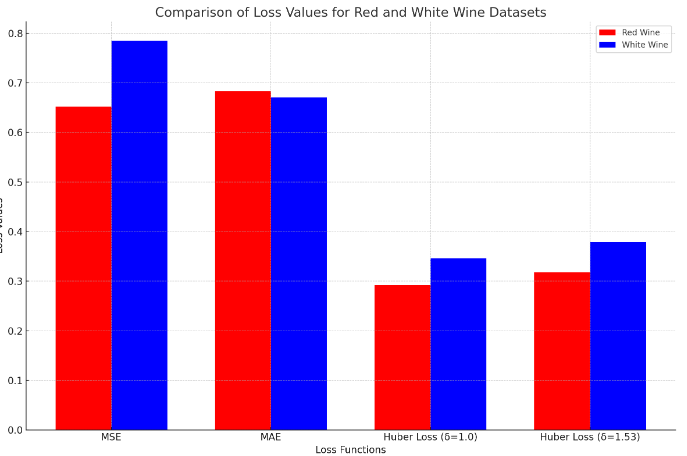
\includegraphics[width=0.75\textwidth]{Graph.png}
    \caption{Bar chart comparison of loss function values for red and white wine datasets.}
    \label{fig:loss_functions_graph}
\end{figure}

\begin{figure}[H]
    \centering
    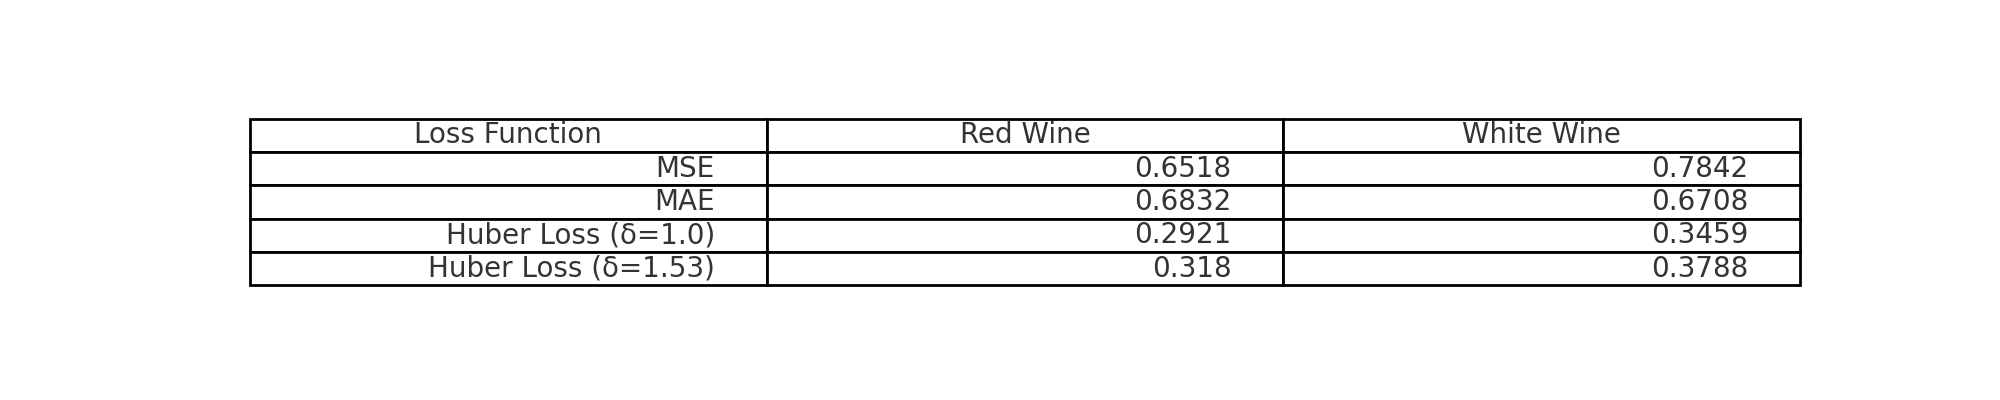
\includegraphics[width=0.75\textwidth]{Sheet.png}
    \caption{Tabulated loss values for MSE, MAE, and Huber Loss with different delta values for red and white wine datasets.}
    \label{fig:loss_functions_sheet}
\end{figure}

The results demonstrate that the choice of loss function significantly impacts the performance metrics of regression models. The Huber Loss with a delta of 1.53 provided a balanced approach to penalizing outliers, as evidenced by its intermediate values between the MSE and MAE. This suggests that Huber Loss could be particularly useful in scenarios where the data contains outliers, as it combines the properties of both MSE and MAE to deliver a robust performance.


\paragraph{Discussion}

This research has systematically investigated the impact of loss function selection on the performance of regression models, specifically within the context of predicting wine quality. We have demonstrated that the Mean Squared Error (MSE), Mean Absolute Error (MAE), and Huber Loss each uniquely influence model outcomes, with the Huber Loss emerging as a robust intermediary that combines the sensitivity of MSE with the outlier resistance of MAE. Our contribution lies in the empirical validation of these loss functions, providing a nuanced understanding that aids in the strategic choice of loss functions to improve model predictions.


The central research question—how the choice of loss function influences the statistical properties of regression models—has been addressed through rigorous analysis. The MSE was found to be less robust to outliers, potentially leading to overfitting to anomalous data points. The MAE offered consistency despite the presence of outliers, and the Huber Loss presented an optimized solution that adapts to the data's inherent variability. The research underscores the critical nature of loss function selection, which is not merely a technical detail but a fundamental aspect that dictates model reliability and validity.


While the study provides valuable insights, it is confined by its scope. The datasets used, derived from red and white wine quality assessments, may not encapsulate the complexity of more heterogeneous data encountered in other domains. Additionally, the study focuses on linear regression models, and the applicability of the findings to non-linear models remains to be thoroughly examined.


Future research should aim to extend the analysis to a broader array of datasets, particularly those with higher dimensionality and complexity. Moreover, exploring the interplay between loss functions and non-linear models, such as those found in deep learning, could yield further valuable insights. The adaptability of the Huber Loss's delta parameter also presents an avenue for exploration, where machine learning techniques could be employed to dynamically adjust this parameter in response to dataset characteristics.


\bibliography{refs}
\bibliographystyle{plainnat}


\end{document}
